\section{Test effettuati} %TODO Graziano, Federica, Carlo i test effettuati da voi
In questa sezione si elencano i test effettuati per il sito in esame.
Per i test di accessibilità eseguiti in remoto, il sito è stato caricato su
GitHub Pages.

\subsection{Validazione XHTML} %DONE
Ogni pagina è stata validata con il tool offerto da W3C all'indirizzo
\texttt{http://validator.w3.org/\#validate\_by\_uri}, con il risultato che
le seguenti pagine non sono valide:
\begin{enumerate}
\item pagina principale del sito;
\item pagina descrittiva di un libro (generata tramite CGI).
\end{enumerate}

\subsection{Validazione CSS} %DONE
Ogni foglio di stile CSS è stato validato con il tool offerto da W3C
all'indirizzo
\texttt{https://jigsaw.w3.org/css-validator/\#validate\_by\_input}, non
trovando alcuna scorrettezza nel codice.

\subsection{Cynthia Says} %DONE
Uno dei tool che è stato utilizzato per controllare l'accessibilità delle
pagine è Cynthia Says, inserendo l'URL di ogni pagina caricata su GitHub Pages
e richiedendo la conformità a WCAG 2.0 AAA.
Di seguito vengono riportati i risultati ottenuti per \textbf{tutte} le pagine
del sito:

\begin{table}[h!]
\begin{center}
\begin{tabular}{ | l | c | }
  \hline
  Conformità & Esito \\
  \hline
  WCAG 2.0 A & Non conforme \\
  \hline
  WCAG 2.0 AA & Non conforme \\
  \hline
  WCAG 2.0 AAA & Non conforme \\
  \hline
\end{tabular}
\caption{Conformità allo standard WAI 2.0 X WCAG}
\end{center}
\end{table}

Le pagine del sito non sono conformi a WCAG 2.0 A, come detto nella sezione
\ref{sec:accessibilita}.

\subsection{WAVE} %DONE
WAVE (Web Accessibility Evaluation Tool) è uno strumento offerto da
\textit{WebAIM} (WEB Accessibility In Mind) per verificare l'accessibilità
delle pagine. Questo strumento analizza una pagina e fornisce errori,
avvertimenti (warnings), caratteristiche positive, struttura basilare di una
pagina e indicazioni sul contrasto.

Tramite i controlli effettuati, sono stati rilevati gli stessi errori
descritti nella sezione \ref{sec:accessibilita}, confermando la non-conformità
al grado WCAG 2.0 A.

WAVE ha inoltre rilevato degli errori di contrasto dovuti al colore giallo
delle intestazioni sopra sfondo bianco (presente di default in assenza
dell'immagine di background). Tuttavia, questa segnalazione viene ritenuta un
falso positivo in quanto il foglio di stile prevede un bordo nero intorno al
titolo.

\subsection{Vischeck} %DONE
Vischek è uno strumento che permette di visualizzare immagini e pagine web
come le vedrebbe una persona che presenta deficit visivi quali:
\begin{itemize}
\item \textbf{Deuteranopia}: una forma di deficit di colore rosso/verde
\item \textbf{Protanopia}: un'altra forma di deficit di colore rosso/verde
\item \textbf{Tritanopia}: una forma di parziale o insufficiente
discriminativa per il blu e il violetto
\end{itemize}
A causa del momentaneo malfunzionamento dello strumento per analizzare le
pagine web, si è provveduto all'analisi tramite l'utilizzo di screenshot. Sono
state analizzate tutte le singole pagine e di seguito portiamo una sola
immagine abbastanza significativa per la comprensione dei casi legati ai
deficit visivi.

\begin{figure}[H]
\begin{minipage}{0.45\textwidth}
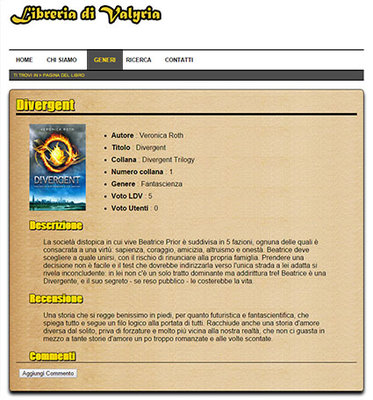
\includegraphics[width=\linewidth]{images/vs_originale.jpg}
\subcaption{Pagina originale (nessun deficit visivo presente)}
\end{minipage}
\hspace{\fill}
\begin{minipage}{0.45\textwidth}
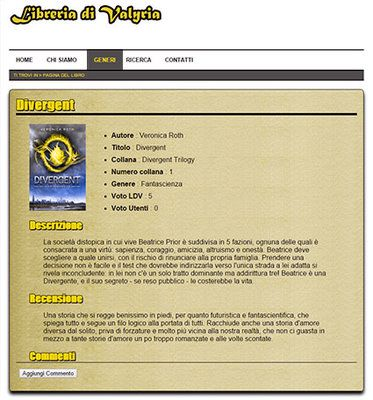
\includegraphics[width=\linewidth]{images/screen/deuteranope.jpg}
\subcaption{Deuteranopia}
\end{minipage}
\vspace*{0.5cm}
\begin{minipage}{0.45\textwidth}
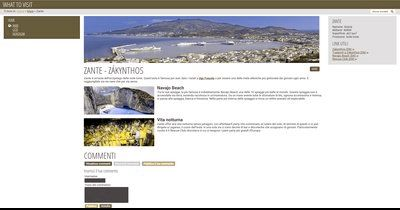
\includegraphics[width=\linewidth]{images/screen/protanope.jpg}
\subcaption{Protanopia}
\end{minipage}
\hspace{\fill}
\begin{minipage}{0.45\textwidth}
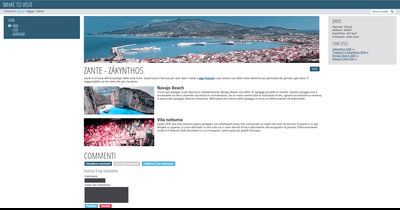
\includegraphics[width=\linewidth]{images/screen/tritanope.jpg}
\subcaption{Tritanopia}
\end{minipage}
\caption{Test con Vischek sulla pagina relativa al singolo libro}\label{multiavp}
\end{figure}

Per quanto riguarda deuteranopia e protanopia, la visualizzazione del sito è
pressochè identica rispetto all'originale e si differenzia solamente quando si
tratta di visualizzare diverse copertine di libri, quando invece si parla di
tritanopia allora si nota un differente modo di vedere gli elementi comuni a
tutte le pagine del sito che comunque rimangono accessibili in ogni caso.

\subsection{Visualizzazione in Bianco/Nero} %DONE
Abbiamo anche esaminato il sito web con una visualizzazione in scala di grigi notando come alcuni elementi non vengano visualizzati al meglio.

\begin{figure}[H]
\begin{minipage}{0.45\textwidth}
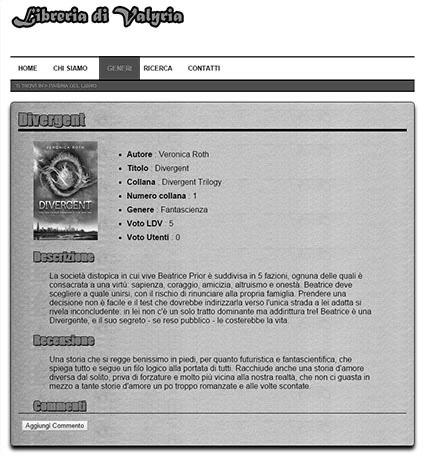
\includegraphics[width=\linewidth]{images/bn_originale.png}
\subcaption{Pagina intera}
\end{minipage}
\hspace{\fill}
\begin{minipage}{0.45\textwidth}
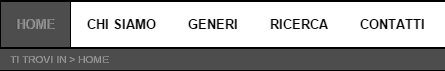
\includegraphics[width=\linewidth]{images/bn_headerbreadcrumb.jpg}
\subcaption{Navigation list e breadcrumb}
\end{minipage}
\vspace*{0.5cm}
\begin{minipage}{0.45\textwidth}
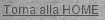
\includegraphics[width=\linewidth]{images/bn_tornahome.jpg}
\subcaption{Link visitato in \texttt{accesso.html}}
\end{minipage}
\hspace{\fill}
\begin{minipage}{0.45\textwidth}
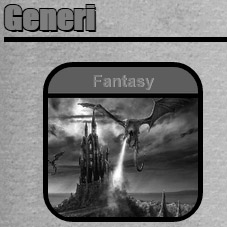
\includegraphics[width=\linewidth]{images/bn_h2etitoli.jpg}
\subcaption{Schede di generi e titoli}
\end{minipage}
\caption{Visualizzazione pagine in scala di grigi}\label{multiavp}
\end{figure}

Dalle figure sovrastanti si può notare come vengono visti alcuni elementi
quando si effettua una visualizzazione in scala di grigi e come questi a
volte non siano accessibili.

Ciò si verifica nel caso di link già visitati in pagine come
\texttt{accesso.html} o \texttt{registrazione.html}, per tutti i titoli dei
generi presenti in \texttt{generi.html}, o come nel caso di breadcrumb e scheda
selezionata in gran parte delle pagine del sito.

\subsection{Fangs}\label{sec:fangs} %DONE
\textit{Fangs} è un'estensione per i browser che consente di visualizzare un
sito nello stesso modo in cui verrebbe visualizzato da uno screen reader,
fornendo il testo come sarebbe letto da questo dispositivo, la lista delle
intestazioni e la lista dei link presenti nella pagina.

In sintesi, come principali problemi vengono individuati:
\begin{itemize}
\item Le parole straniere lette in italiano;
\item A volte i numeri sono scritti in numero; ciò vuol dire che se l'utente
ha la lingua di default del computer/browser impostata su inglese (come nel
caso di un verificatore) si hanno frasi come ``\textit{La società distopica in
cui vive Beatrice Prior è suddivisa in five fazioni}", mentre in casi simili
un numero dovrebbe essere scritto per esteso;
\item Si vedono i nomi dei file delle immagini anzichè un testo alternativo;
\item Quando presente, il testo delle immagini spesso trasmette poca
informazione, ridondando semplicemente il titolo anzichè rimanere vuoto
(soluzione preferibile alla ridondanza);
\item Le abbreviazioni non vengono estese, diventando potenzialmente
incomprensibili.
\end{itemize}

\subsection{Lynx}\label{sec:lynx} %DONE
Le pagine del sito sono state anche navigate tramite il browser testuale
\textit{Lynx}.

Come principale difetto, non è possibile effettuare l'accesso a funzioni come
accesso e registrazione, poichè tutti i pulsanti hanno la sottomissione
dell'input gestita tramite JavaScript, quindi per testare tutte le pagine, si è
provveduto a fare una copia dei file una volta loggati tramite browser e poi
ogni pagina è stata aperta con Lynx.

Gli errori rilevati sono gli stessi discussi nelle altre sezioni.
